\documentclass[12pt,a4paper]{report}
\usepackage{graphicx}
\usepackage{url}
\usepackage{amsmath}
\usepackage[utf8]{inputenc}
\usepackage[english]{babel}
\usepackage[left=3cm,right=3cm,top=3cm,bottom=3cm]{geometry}
\usepackage[colorlinks=true,allcolors=blue]{hyperref}
\usepackage{hyperref,cleveref}
\usepackage{cite}
\usepackage{caption}
\usepackage{subcaption}
\usepackage{siunitx}
\usepackage{tabularx}

\begin{document}
	\title{SARAO Virtual Evaluation Worksheets for Graduate Trainee Engineer in 2021 for the RFI team.\\ [1cm]
		by Tankiso H. Moso\\[4cm]	
		Submitted on	
	}
	
	\maketitle

	
	\chapter{Introduction}
	\section{Background}
	A virtual worksheet was presented to potential candidates/graduates by the South African Radio Astronomy Observatory (SARAO) to test their knowledge of SARAO's various aspects; this was an effort to recruit candidates 2021 SARAO graduate programme. The worksheet was dependant on which department a candidate was shortlisted. This document presents the worksheet tasked with the candidates shortlisted under the Radio Frequency Interference (RFI) team. A period of $\sim$ two weeks was given to shortlisted candidates to complete and submit the tasks on the worksheet and further write a report based on the tasks.
	
	\section{Overview}
	
	Radio astronomy was born when Karl Jansky designed an antenna that operated at $\sim$ 20 MHz (15 m wavelength). The frequency-wavelength relation 
	
	\begin{equation}
	\lambda = \frac{c}{f}
	\end{equation}
	
	relates the wavelength $\lambda$ to essential factors, which are c, the speed of light \SI{3e8}{\metre\per\second}, and f, the frequency in Hz. The antenna that he designed was intended for communication systems research. He further found radio radiation from the Galactic Center at the operating frequency.\\
	
	It should be well noted that with every antenna design lies observational challenges that include RFI. RFI can be human-made or due to instrumental systematics; that is why electronic equipment/components need to undergo measurements to understand the interference emitted or absorbed. The measurements/tests are done using the electromagnetic compatibility (EMC) chamber. Faraday cage, anechoic chamber, and reverberation chamber may be needed depending on the type of tests being done.\\
	
	During these tests, specific equipment is needed where the widely used piece of equipment is the spectrum analyzer. The spectrum analyzer can store the measured results in various file extensions. The most commonly used is the .csv, which is later imported to the desired programming platform, plotted and analyzed accordingly. Since it is a learning curve, a candidate may expect any other form of task that may not be mentioned but aligns with the department's line of work.
	
	\section{Specifications}
	
	The worksheet specifications can be found at:  \href{https://github.com/Casablanca25273/Worksheet}{New RFI Graduate Virtual Evaluation - Worksheet.pdf}
	
	
	They are also detailed below.
	
	\subsection*{Radio Astronomy Worksheet}	
	
	You are the Science Reporter for a large media house. Your (tough) editor have heard about the MeerKAT project and asked you to investigate and write a story for publication; your story should answer the following questions:
	\begin{enumerate}
		\item What is this MeerKAT story?
		\item Why is it being built in the remote Northern Cape and not close to a city such as Cape Town?
		\item What is it going to do (Science)?
		\item How does it work?
		\item Who is funding this, and how much is it going to cost?
		\item When did the building start, and how far are they?
		\item When is it going to be finished?
		\item What is the benefit/impact on the environment/local community?
		\item Get some nice photos to show what it looks like
	\end{enumerate}	
	
	Handy Links:
	\begin{itemize}
		\item \url{https://www.ska.ac.za}
		\item \url{https://www.skatelescope.org}
		\item \url{https://en.wikipedia.org/wiki/Square\textunderscore Kilometre\textunderscore Array}
	\end{itemize}
	
	\subsection*{EMC Chamber Worksheet}
	
	\begin{enumerate}
		\item What is a Faraday cage?
		\item Is a Microwave oven a Faraday cage?
		\item What can a Faraday cage be used for in the radio telescope environment?
		\item What is an Anechoic chamber?
		\item What is a Reverberation Chamber?
		\item What can an Anechoic chamber/ Reverb chamber be used for in a radio telescope environment?
	\end{enumerate}
	
	Handy Links:
	\begin{itemize}
		\item \url{https://en.wikipedia.org/wiki/Faraday\textunderscore cage}
		\item \url{https://en.wikipedia.org/wiki/Microwave\textunderscore oven}
		\item \url{https://en.wikipedia.org/wiki/Anechoic\textunderscore chamber}
		\item \url{https://en.wikipedia.org/wiki/Electromagnetic\textunderscore reverberation\textunderscore chamber}
	\end{itemize}
	
	\subsection*{Python Worksheet}
	
	A part of what the RFI team of SARAO does to limit the amount of RFI on the SKA SA site is to characterize the emissions from a device that needs to be used on-site before it goes to the site. The characterization of the device is done at an EMC facility like the anechoic chamber at Houwteq or the reverberation chamber at SARAO's offices in Observatory, Cape Town.\\
	
	An example of a system characterized in the SARAO RFI Reverberation chamber is the internal electronics used in the HERA project nodes. The system was characterized by placing it inside the reverberation chamber, having the stirrer paddles rotate at a speed of 15 degrees a second, and setting the Tektronix RSA 5115B spectrum analyzer to max-hold. Two measurements were done. One with the HERA electronics running and one with the HERA electronics turned off, in other words, the background of the chamber. Take a look at the files of these two measurements, which are available using the following link: \href{https://github.com/Casablanca25273/Worksheet}{2020\textunderscore 10\textunderscore 07\textunderscore Hera\textunderscore Node\textunderscore 18\textunderscore maxhold\textunderscore 1kHz}.\\
	
	You are one of the graduate students working at SARAO and are tasked with the following:
	
	\begin{enumerate}
		\item Use Python to plot the raw data of the measurements on the same plot.
		\item Use Python to plot the corresponding E-Field at 1 m using the following file (\href{https://github.com/Casablanca25273/Worksheet}{ProcHeraAux.csv}). This file includes the following: Frequency (MHz), Pow2EfieldFactor, E\textunderscore Spec, and E\textunderscore Cont. 
		
		The Pow2EfieldFactor should be used to take the spectrum analyzer's data and calculate the corresponding E-Field at 1 m by adding it to power measured from the spectrum analyzer.
		
		The E\textunderscore Spec and E\textunderscore Cont are the threshold levels that devices must adhere to for a distance of 500 m and an E-Field measured at 1 m, like in this case.
		
		\item Use the plot to determine and fill in the following:
	\end{enumerate}
	
	\begin{itemize}
		\item At which frequency is the maximum emission?
		\item What is the E-Field strength @ 1 m of the maximum emission?
		\item How much shielding (dB) would the node enclosure need to pass the E\textunderscore Spec threshold?
	\end{itemize}
	
	\subsection*{Arduino Worksheet}
	
	To be viewed at the link provided earlier in the section.
	
	\href{https://github.com/Casablanca25273/Worksheet}{New RFI Graduate Virtual Evaluation - Worksheet.pdf}
	
	
	
	
	
	
	
	
	
	
	
	
	
	
	
	
	
	\chapter{Solutions to the worksheet}	
	
	\section{Radio Astronomy}
	
	In this section, an article about the Meerkat telescope is broken down to answer all the questions that were provided in section 1.3.\\
	
	{\noindent \large Meerkat, the World Class Science Instrument}	
	
	\begin{figure}[h]
		\centering
		\includegraphics[width=\linewidth]{Meerkat_1000p}
		\caption{The Meerkat telescope that consists of sixty-four dishes and a precursor of the Square Kilometre Array (SKA). Image Credit: SARAO}
		\label{fig:Meerkat}
	\end{figure}	 
	
	The Meerkat radio telescope is an interferometric array based in the South African Karoo region in the Northern Cape province, a precursor of the Square Kilometre Array. The array consists of sixty-four antennas conduct astronomical measurements from 580 MHz to 14.5 GHz, with a maximum baseline length of \SI{\sim 8 }{\kilo \meter}. Each antenna comprises the main reflector of 13.5 m effective diameter and a 3.8 m diameter sub-reflector.
	
	The main reflector of a radio telescope collects the electromagnetic radiation from cosmic radio sources to the sub-reflector. Further, it transmits the radio waves to the feed horn of the receiver.	All the antennas consist of up to four receivers and four digitizers and can be steered to the selected receiver observation frequency. The captured electromagnetic waves are then converted to a voltage signal and amplified by cryogenic receivers. The analog to digital converter within the digitizers converts the radio frequency voltage signals to the digital signals.\\
	
	At the digitization stage, the signals are also sampled at a rate of 1 712 million samples every second; the signals are then sent to the correlator at the Karoo Array Processor Building (KAPB) using a total of 170 km fiber optic cables. To ensure proper alignment of signals from all receptors, the signals are synchronized to the same clock. The correlator coherently adds the signals from all the antennas to form several narrow, high sensitivity beams used for pulsar science. The data is stored at the KAPB, and some of the data is transferred to Cape Town via fiber connection. Several sensors (temperature sensors, weather conditions, power consumption, etc.) are embedded in the telescope's control and monitoring system. \\
	
	
	\begin{figure}[h!]
		\centering
		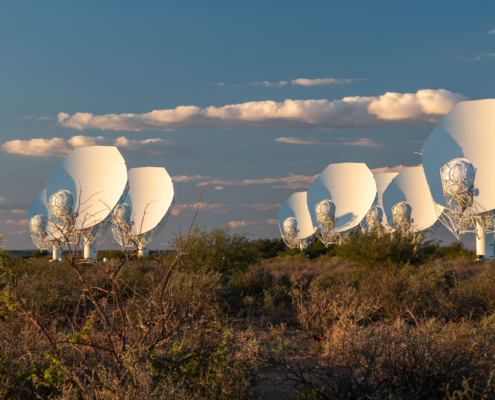
\includegraphics[width=0.7\linewidth]{2018-MeerKAT-5-495x400}
		\caption{Another photograph of the Meerkat radio telescope at the Karoo site. Image Credit: SARAO}
		\label{fig:2018-MeerKAT-5-495x400}
	\end{figure}
	
	The Meerkat telescope's commissioning began in 2012 and was finished in 2018 at a specifically chosen site in the Karoo for its RFI-quiet environment and favorable physical site characteristics. The instrument has already given the world a glimpse into the star-formation history of the universe. The other science topics that Meerkat has or will reveal include "radio pulsar timing, Looking at the Distant Universe with the MeerKAT Array (LADUMA), MeerKAT Search for Molecules in the Epoch of Re-ionisation (MESMER), MeerKAT Absorption Line Survey, MeerKAT HI Observations of Nearby Galactic Objects: Observing Southern Emitters (MHONGOOSE), Transients and Pulsars with MeerKAT (TRAPUM), Galaxy formation and evolution in the cluster environment, MeerKAT High-Frequency Galactic Plane Survey (MeerGAL), MeerKAT International GigaHertz Tiered Extragalactic Exploration Survey (MIGHTEE), The Hunt for Dynamic and Explosive Radio Transients with MeerKAT (ThunderKAT), and Very Long Baseline Interferometry" according to SARAO.\\
	
	The SKA SA has invested in the Northern Cape communities by funding, empowering, and encouraging the youth/learners to pursue science, technology, engineering, and mathematics fields, supporting local contractors and community programs.
	
	The Meerkat project team acknowledges the South African Department of Science and Innovation, through the National Research Foundation and SARAO for investing more than R760 million in the precursor of the SKA.
	
	
	{\section{Appendix B: EMC Chamber}
		
		The RFI team of SARAO uses the electromagnetic compatibility (EMC) chamber to characterize the device's performance before it is allowed to be used on the SKA SA site. The characterization is done to prevent unwanted emissions from devices and considering that the MeerKat telescope has a high sensitivity that can be picked up from raw data of observations. To avoid RFI emission from devices, an EMC chamber is used, and it is defined as equipment to assess the performance of electronic devices under certain conditions and settings. The results are then compared to the standard regulations to analyze radiated and conducted radio frequency (RF) emissions and immunity. The EMC chambers can be categorized as Faraday cage, anechoic chamber, and reverberation chambers. Further description is provided in the sections that follow.
		
		\section*{Faraday Cage}
		A Faraday cage is an enclosure used to shield electronic components/equipment from radio frequency interference (RFI) is called a Faraday cage. Faraday cages are also used for lightning protection against humans. The continuous covering of a mesh of conductive material may form a Faraday cage. The operation of a Faraday cage is caused by an external electric field, which causes the electric charges within the enclosure's conducting material to be distributed to cancel the field's effect in the cage's interior.
		
		\section*{Microwave Oven as a Faraday Cage}
		
		A Microwave oven is a hybrid Faraday cage. The microwave glass window consists of a series of holes placed in a metal screen to act as one side of the Faraday cage. The energy given off by the electromagnetic pulse is kept in the microwave's three conductive metal walls and metal mesh viewing window.
		
		\section*{Faraday Cage uses in a Radio Telescope Environment}
		
		In a radio telescope environment, someone can use it for performing RFI emission measurements from several electronic components/ equipment.
		
		\section*{Anechoic Chamber}
		
		\begin{figure}[h!]
			\centering
			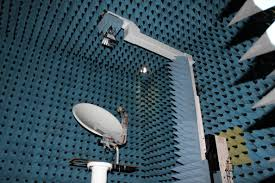
\includegraphics[width=\linewidth]{anechoic}
			\caption{Anechoic chamber with a device under test (parabolic dish antenna)}
			\label{fig:anechoic}
		\end{figure}
		
		An anechoic chamber, as shown in Figure~\ref*{fig:anechoic} is a room covered with radiation absorbent material (RAM) to avoid the reflected RF radiation from surfaces. It is also designed in such a way that it shields inward interferences.
		
		\section*{Reverberation Chamber}
		
		\begin{figure}[h!]
			\centering
			\includegraphics[width=\linewidth]{reverb}
			\caption{Internal of the reverberation chamber with the stirrers clearly visible.}
			\label{fig:reverb}
		\end{figure}
		
		
		A reverberation chamber, as shown in Figure~\ref*{fig:reverb} is an environment/room for measuring equipment or systems' capability to perform adequately in their electromagnetic environment without introducing unbearable electromagnetic interference to anything in that environment. Stirrers are used in reverberation chambers to reduce the spatial dispersion of the electrical and magnetic field strength.\\
		
		\section*{Uses in Radio Telescope Environment}
		
		This specialized equipment can be used in a radio telescope environment to enclose the device under test (antenna or radar) to measure the radiation pattern, gain, RFI, and performance under specified conditions.
		
		{\section{Appendix B: Python}
			
			During DUT characterization, a Tektronix RSA 5115B spectrum analyzer was used. The measurements were conducted in the SARAO reverberation chamber, measuring the internal electronics used in the Hydrogen Epoch of Reionization Array (HERA) project nodes. The electronics were placed inside the reverberation chamber, having the stirrer paddles rotate at a speed of 15 degrees a second and setting the spectrum analyzer to max-hold. Two measurements were done. One with the HERA electronics running shown in Figure~\ref*{fig:HERA} by the blue plot labeled HERA on, and one measurement was with the HERA electronics turned off; in other words, the background of the chamber shown in Figure\ref*{fig:HERA} by the green plot labeled HERA off. 
			
			The two measurement plots were saved on the spectrum analyzer as .csv files, and they were plotted using Python programming language. The Python script can be found on \href{https://github.com/Casablanca25273/Worksheet}{maxhold.py}. The difference between the two measurements was also plotted as shown in Figure~\ref*{fig:Diff}.\\
			
			\begin{figure}[h!]
				\centering
				\begin{subfigure}[b]{0.49\textwidth}
					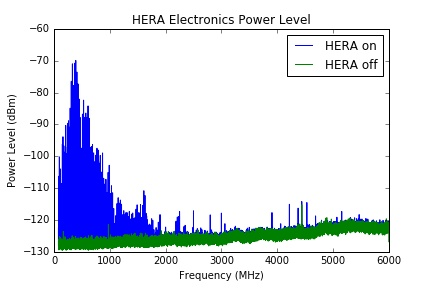
\includegraphics[width=\textwidth]{HERA.jpeg}
					\caption{Plot of the two measurements that were done. One with the HERA electronics running (HERA on) and one with the reverberation chamber backround (HERA off).}
					\label{fig:HERA}
				\end{subfigure}
				\hfill
				\begin{subfigure}[b]{0.49\textwidth}
					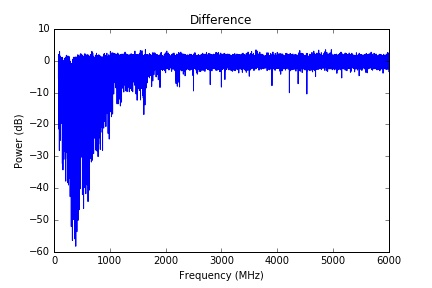
\includegraphics[width=\textwidth]{Diff.jpeg}
					\caption{Plot that shows the difference between the two measurements that were taken in the reverberation chamber at SARAO.}
					\label{fig:Diff}
				\end{subfigure}
				\caption{Reverberation chamber measurements of the HERA electronics.}
			\end{figure}
			
			Further measurements were done that correspond to the first two measurements, and they were also saved as .csv file and were further plotted and analyzed accordingly. \href{https://github.com/Casablanca25273/Worksheet}{ProcHERAAux.py} is a Python script that was written to analyze and answer questions from the specifications. In Figure~\ref*{fig:E-Field}, the corresponding E-field at 1 m was plotted labeled as HERA, the Pow2EfieldFactor shown in Figure~\ref*{fig:powtoefield} was used to take the data from the spectrum analyzer and calculate the corresponding E-Field at 1 m by adding it to power measured from the spectrum analyzer.
			
			\begin{figure}[h!]
				\centering
				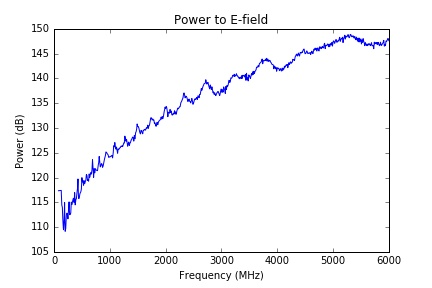
\includegraphics[width=0.7\textwidth]{powtoefield.jpeg}
				\caption{Plot of the power to e-field that was measured and deduced from the .csv file provided.}
				\label{fig:powtoefield}
			\end{figure}
			
			Figure~\ref*{fig:E-Field} also shows E\textunderscore Spec, E\textunderscore Cont, which are the threshold levels that devices must adhere to for a
			distance of 500 m and an E-Field measured at 1 m. The plot labeled Background is a plot of the background of the E-field, which is the sum of the Pow2EfieldFactor and power level of the HERA off shown by Figure~\ref*{fig:HERA} and Figure~\ref*{fig:shield} shows the shielding needed by the node enclosure to pass the E\textunderscore Spec threshold. 
			
			\begin{figure}[h!]
				\centering
				\begin{subfigure}[b]{0.49\textwidth}
					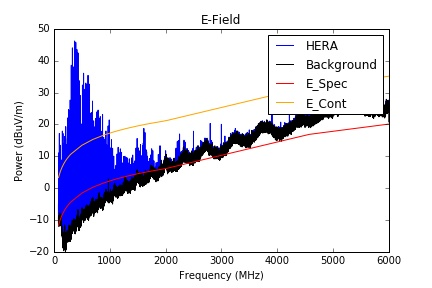
\includegraphics[width=\textwidth]{E-Field.jpeg}
					\caption{Four plots of the e-fielf on the same set of axes. HERA, Background, E\textunderscore Spec, and E\textunderscore Cont.}
					\label{fig:E-Field}
				\end{subfigure}
				\hfill
				\begin{subfigure}[b]{0.49\textwidth}
					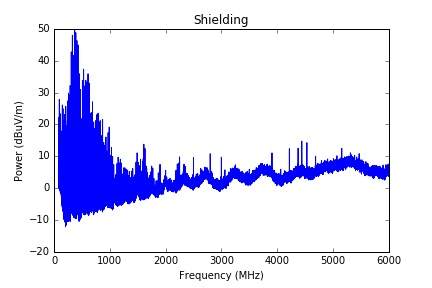
\includegraphics[width=\textwidth]{shield.jpeg}
					\caption{Plot showing the shielding needed by the node enclosure to pass the E\textunderscore Spec threshold}
					\label{fig:shield}
				\end{subfigure}
				\caption{E-field measurements that were done corresponding with the first two measurements.}
			\end{figure}
			
\section{Appendix B: Arduino}

Arduino is an open-source electronics platform based on hardware and software. Arduino boards can read inputs and turn them into an output, for example, turning on an LED. The user controls the board by sending instructions to it. Arduino programming language (based on Wiring) is used, and the Arduino Software (IDE) is based on Processing.	

An Arduino was used to design and build a  traffic light control system using Arduino controllers. Three Arduinos were used, one Arduino as the Main Event Controller (MEC) to schedule the events and two Arduino controllers as Secondary Light Controllers (SLCs) to control the colors of the lights. An Arduino I2C interface was used for communication between the MEC and SLCs.

TinkerCAD was self-taught and used for the two-pole traffic signal simulation. The traffic signal poles were set up, as shown in Table~\ref*{table:1}.

\begin{table}[h!]
	\centering
	\begin{tabular}{| c | c | c | c |} 
		\hline
		Event no. & Duration (seconds) & Pole 1 & Pole 2 \\
		\hline
		1  &  5  & Green & Red  \\
		\hline
		2 & 2 & Yellow & Red  \\
		\hline
		3 & 1 & Red & Red \\
		\hline
		4  &  5  & Red & Green  \\
		\hline
		5 & 2 & Red & Yellow  \\
		\hline
		6 & 1 & Red & Red \\
		\hline
	\end{tabular}
	\caption{Setup of the two traffic signal poles}
	\label{table:1}
\end{table}

Figure~\ref*{fig:DaringAmberis} shows the circuit that was designed and built on TinkerCAD online simulator for two traffic signals using three Arduinos. The leftmost Arduino was setup as SLC1 (\href{https://github.com/Casablanca25273/Worksheet}{daring\textunderscore amberis1.ino}), the middle Arduino was set up as the MEC (\href{https://github.com/Casablanca25273/Worksheet}{daring\textunderscore amberis2.ino}), and the last Arduino was setup as SLC2 (\href{https://github.com/Casablanca25273/Worksheet}{daring\textunderscore amberis3.ino}). Three light-emitting diodes (LEDs) were used on both poles as traffic signal lights. The formula 

\begin{equation}
R = \frac{{V_{s}} - {V_{f}}}{I_{f}}
\end{equation}

was used for calculating the LED series resistors. $V_{s}$ is the supply voltage, $V_{f}$ is the forward voltage, and $I_{f}$ is the forward current of the LED. 

\begin{figure}[h!]
	\centering
	\includegraphics[width=\linewidth]{"Daring Amberis"}
	\caption{TinkerCAD online simulator was used for two traffic signals using three arduinos. The left most arduino was setup as SLC1 the middle arduino was setup as the MEC and the last arduino was setup as SLC2. Three light emitting diodes (LEDs) were used on both poles as traffic signal lights.}
	\label{fig:DaringAmberis}
\end{figure}

\section{Conclusion}
Worksheets A to D were discussed and answered. MeerKat radio astronomy was discussed in detail as an article, EMC chambers were broken down and further discussed. Python and Arduino worksheets were completed with their codes on the GitHub repository.

		
		\end{document}